\section{Introduction}
\label{sec:bw:intro}

The very quality that makes batteries interesting for academic research is concurrently a source of frustration for their practical implementation: each chemistry has a specific physical fingerprint, which leads to unique cycling behaviors, desired or otherwise. The standard suite of electrochemical tools provides a window into the physical changes of each chemistry, but it is at best an abstract representation of the physical changes occurring in the cell. As discussed in Chapter~\ref{ch:dbb}, \textit{in situ} and \textit{in operando} optical~\cite{Ito2011-ir,Gallaway2010-xk}, electron~\cite{Santhanagopalan2014-xh,Karki2014-jj,Radisic2006-zq}, x-ray~\cite{Nelson2012-rq, Chen-Wiegart2013-kh, Liu2013-gi, Marone2013-jh} and neutron scattering~\cite{Manke2007-yj, Armstrong2006-vg, Du2011-up} methods have provided rich data which describe the behavior of idealized cells, but with few exceptions~\cite{gallaway, Senyshyn2012-pz, Rijssenbeek2011-st, Gallaway2015-xy} it has been difficult to directly probe the physical changes in conventional batteries. This is a true detriment to the field, as scaling up cells is not a trivial linear exercise: physical insights into large-scale cells, without the need for expensive equipment such as a synchrotron light source, would be welcome both in academia and in industry.

In this chapter, we present the framework for a non-invasive, \textit{in operando} method that is able to extract a rich data set from numerous battery designs by exploiting a physical truth that underlies all closed electrochemical systems: they are, by design, reactors which redistribute density as a function of SOC in the ideal case and, additionally, as a function of SOH in reality. Regardless of the reaction mechanism (intercalation, dissolution/reprecipitation, phase change, etc.), the density and elastic modulus of an electrode changes as a function of its SOC, and this distribution as well as the rate of change of this distribution can act as a fingerprint of SOH. We use acoustic ultrasonic transducers to probe the changes in density distribution in real time, and provide a model which describes how ultrasonic echoes within an arbitrary cell change as a function of the SOC. The concept for this approach is illustrated for an example cell in Fig.~\ref{fig:bwschem}. In this article we discuss a simple method that may be used with one or two transducers to characterize SOC and SOH. Beyond correlations between density and acoustic signal amplitude, acoustic attenuation will also change as a function of the effective modulus of each layer in the battery.

\begin{figure}[htb]
  \centering
    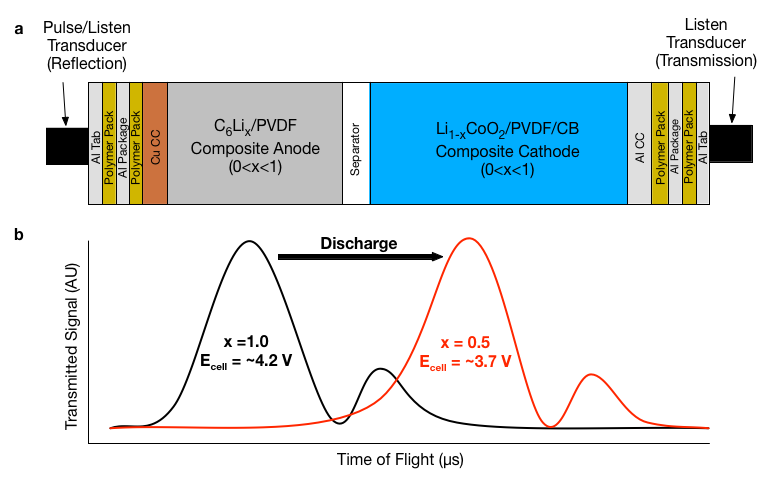
\includegraphics[width=0.8\textwidth]{ch4-bw/images/bwschem.png}
    \caption[Schematic of ultrasonic interrogation of a representative Li-ion battery.]{Schematic of ultrasonic interrogation of a representative Li-ion battery, showing a) a typical battery with the various packaging, current collector, electrode, and separator layers as well as the two acoustic transducers (pulse/listen and listen) used for ultrasonic interrogation and b) an example illustration of the increase in time of flight (ToF) of the transmitted signal as a function of SOC that occurs during discharge.}
    \label{fig:bwschem}
\end{figure}

Recently, there has been significant work correlating static strain at a macroscopic level to SOC and SOH in batteries which exhibit significant volume changes.~\cite{cannarella_ion, cannarella_stress, Deshpande2012-wk, J2014-cd, Cannarella2014-ej} In some cases, the macroscopic strain can be exploited as an actuator.~\cite{Koyama2006-hm} Acoustics have been employed to detect emissions from macroscopic cracking,~\cite{Kircheva2011-ji, Komagata2010-sw, etiemble, Didier-Laurent2008-tt} and microscopic AFM measurements~\cite{Rhodes2010-nr, rhodes} and models have been developed to determine the causes and critical aspects of “electrochemical shock.”~\cite{Woodford2014-tq, Woodford2010-vd, Woodford2012-fq, Woodford2014-gy} While there have been efforts in ultrasonic imaging of full cells, they have focused on the examination of irreversible failure through delamination and cracking.~\cite{Sood2013-bo, Sood2013-yf} Thus far, no efforts have correlated slight-to-moderate mechanical degradation or SOC with ultrasonic interrogation. In this work, we employ acoustic methods that were developed for flaw detection of bulk metals and welds~\cite{Vary1982-dy, Banks1963-vo, Furgason1975-md} to accurately correlate state of charge within a battery to subtle changes within materials and between layers.